% Based on a template created by João Alegria (https://github.com/joao-alegria)
%  and Filipe Pires (https://github.com/FilipePires98)
 
\documentclass[12pt]{article}

\usepackage[english]{babel}
\usepackage[utf8x]{inputenc}

\usepackage{float}
\usepackage{hyperref}
\usepackage{times}
\usepackage{url}

% Images
\usepackage{graphicx}
\graphicspath{{images/}}

% Page dimensions
\topmargin -1.0cm
\oddsidemargin 0.0cm
\textwidth 16cm 
\textheight 23cm
\footskip 1.0cm

% TITLE PAGE CONTENT BEGIN

\title{Assignmnet 1}

\author{
    André Pedrosa [85098], João Abílio [84732]\\
    \\
    Recuperação de informação\\
    \normalsize{Departamento de Eletrónica, Telecomunicações e Informática}\\
    \normalsize{Universidade de Aveiro}\\
}

\date{16 de outubro de 2019}

% TITLE PAGE CONTENT END

\begin{document}

\baselineskip18pt

\maketitle

\section{Introdução}
Este relatório apresenta uma explicação do trabalho desenvolvido
para o primeiro assignment da disciplina "Recuperação de Informação",
explicando as decisões tomadas e o funcionamento da solução.

A linguagem de programação usada foi o Java e o programa desenvolvido
tem como objetivo indexar uma coleção de documentos, criando um index
invertido que faz a associação entre termos e os documentos nos quais
aparece-se.

No fim serão apresentados resultados às questões colocadas no enunciado
do assignment com o index resultante do programa.

Devido ao elevado número de classes criadas, o diagrama de classes vai ser
dividido em vários que vão sendo apresentados ao longo do relatório. Estes
diagramas foram gerados através do IDEA IntelliJ, consequentemente em anexo
é disponibilizada a legenda da convenção usada.

\section{Decisões de implementação}
Durante a implementação deste assignment não foi dada atenção a questões de memória,
no entanto seguimos uma aproximação de iterativa em que o pedido de informação
(conteúdo de ficheiros a ler, documentos, ...) pode ser condicionado segundo as
limitações de memória em implementações futuras facilmente.

Partes da nossa solução foram moduladas já a pensar nos futuros assignments,
possibilitando a indexação ser feita em diferentes formatos de documentos e a informação
presente no index poder variar.

\section{Data Flow}
\begin{figure}[h]
  \center
  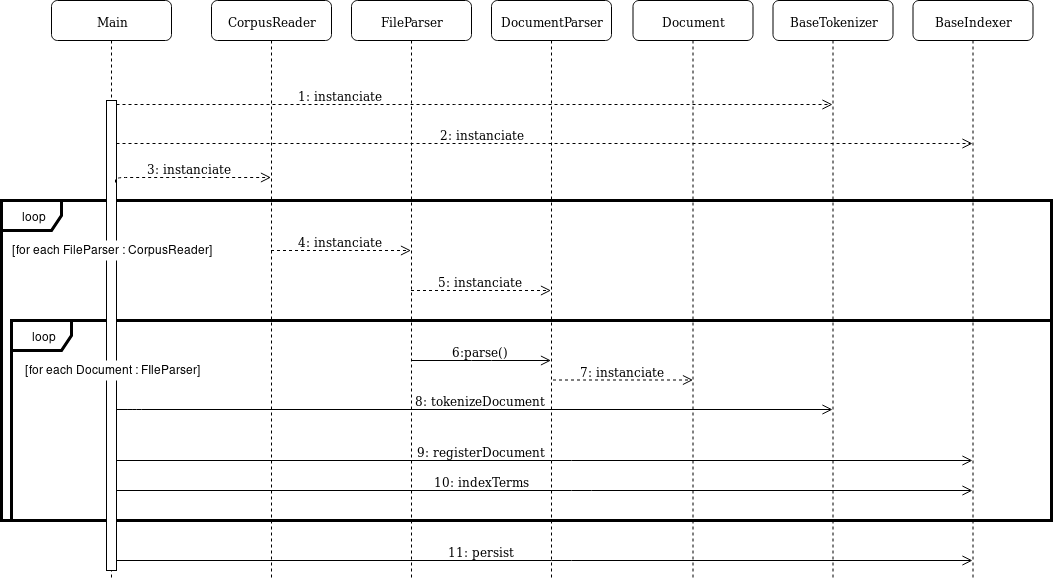
\includegraphics[width=17cm]{sequenceDiagram.png}
  \caption{Diagrama de sequência da solução}
\end{figure}

O pipeline da nossa solução está implementado no método main da classe
Main. Primeiramente, aqui é instanciado o respetivo Tokenizer e o Indexer.

O Main instância um classe do tipo CorpusReader, sobre a qual fará um for each, no
qual em que cada iteração receberá um FileParser. O Main itera também com um
for each sobre o FileParser. Para cada ciclo do último for each mencionado, a classe
FileParser está continuamente a ler linhas do ficheiro até ter um documento
válido. Neste momento, passa o conteúdo lido a um DocumentParser que extrai
do documento a informação importante (identifier e outros campos) criando
uma classe Document, a qual será devolvida para o for each no método main.

Este documento é registado no index (associar um document id ao identifier do
documento) e posteriormente os seu termos são indexados.

Por último, as estruturas internas do index são escritas para disco.

\section{Packages}

\begin{figure}[H]
  \center
  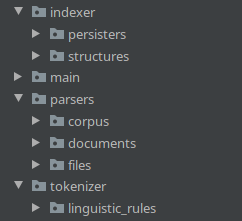
\includegraphics[width=6cm]{packages_all.png}
  \caption{Árvore de packages da solução}
\end{figure}

Nesta secção vai ser apresentada uma descrição para cada package presente na
nossa solução apresentando as principais classes e os seus principais métodos. 

\subsection{main}

Neste package encontra-se a classe com o método main onde é feito o
processamento dos argumentos e opções do programa e onde é definido o
pipeline de processamento.

Tem ainda a classe responsável por consultar o index de maneira a
obter os dados para responder às questões propostas no enunciado.

\subsection{parsers}
Neste package encontram-se as classes com a responsabilidade de fazer
o processamento do corpus. Este processamento engloba percorrer a pasta do
corpus, abrir os vários ficheiros, retirar os documentos dos ficheiros e
recolher as as partes a indexar dos documentos.

\subsubsection{parsers.corpus}
\begin{figure}[h]
  \center
  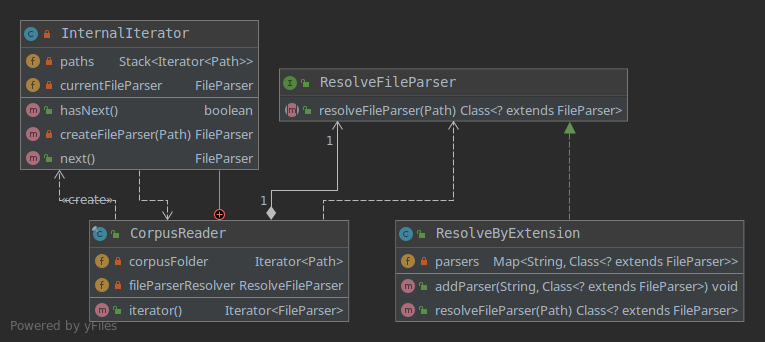
\includegraphics[width=12cm]{packages_parsers_corpus.png}
  \caption{Diagrama de classes do package \it parsers.corpus}
\end{figure}

Package onde é feita a iteração sobre os ficheiros a serem indexados, criando as classes
necessárias para as classes seguintes poderem ler destes ficheiros.

A classe CorpusReader implementa a interface Iterable o que permite receber os ficheiros
a processar numa aproximação do tipo iterativa, como foi mencionado anteriormente. Quando
é chamado o método {\it hasNext} do iterador da classe CorpusReader, a pasta do corpus
é percurida recursivamente (usando uma stack para continuar a recursividade nas chamadas
seguintes) até encontrar um ficheiro, o qual será retornado na próxima chamada do método
{\it next}.

Nesta altura é necessário escolher o FilePaser (mencionado mais à frente) adequado para
o tipo de ficheiro para isso a classe CorupusReader tem uma interface ResolveFileParser
que é responsável por fazer a associação entre o ficheiro e FileParser adequado. Para este
assignment foi desenvolvido uma classe que escolhe o FileParser segundo a extensão do ficheiro.


\subsubsection{parsers.files}
\begin{figure}[h]
  \center
  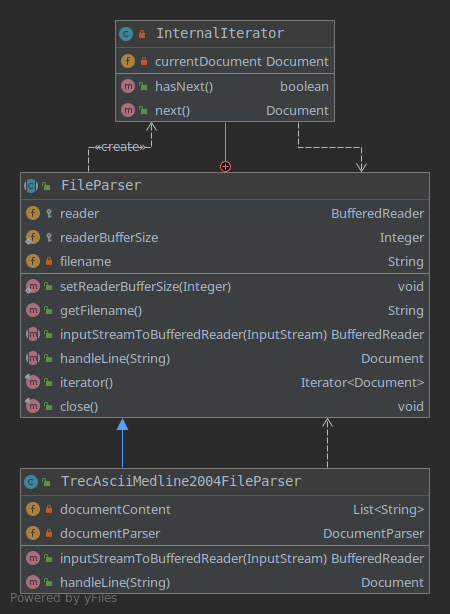
\includegraphics[width=6cm]{packages_parsers_files.png}
  \caption{Diagrama de classes do package \it parsers.files}
\end{figure}

Mais uma vez, para obtermos os documentos de cada ficheiro seguimos uma aproximação
iterativa, em que a classe FileParser implementa a interface Iterable. O método
{\it hasNext} do iterador da classe FileParser lê linha a linha de um BufferedReader
até que o método {\it handleLine} retorne uma referência para um objeto do tipo Document
(do package parsers.documents) não nula, a qual será retornada na próxima chamada do
método {\it next}.

Para cada formato de ficheiro diferente deverá ser criada uma classe descendente da classe
FileParser, implementando o método {\it handleLine} que retorna objetos Document quando
as linhas lidas até ao momento completam um documento, e o método {\it inputStreamToBufferedReader},
que transforma uma InputStream num BufferedReader permitindo inserir os necessários wrappers.
Este último método permite abrir todos os ficheiros da mesma maneira e deixando para os FileParsers
a responsabilidade de criar os necessários wrappers. Exemplo: \(InputStream >
GZIPInputStream > InputStreamReader > BufferedReader\).

\subsubsection{parsers.documents}
\begin{figure}[h]
  \center
  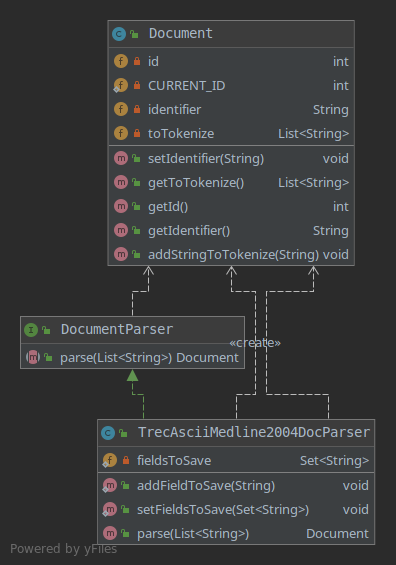
\includegraphics[width=6cm]{packages_parsers_documents.png}
  \caption{Diagrama de classes do package \it parsers.documents}
\end{figure}

O documento devolvido no método {\it handleLine} resulta do parsing do conteúdo do
documento por um DocumentParser. O objetivo desta classe é retirar do conteúdo do documento
a informação necessária para a indexação e criar um objeto Document associado. Este objeto
tem um id que é incrementado a cada Document criado, não havendo ids repetidos, um identifier,
que é utilizado para fazer a associação do id para ao documento, e apresenta uma lista do
conteúdo a ser tokenizado e posteriormente indexado.

Para cada formato diferente de documentos deverá ser criada uma classe descendente da classe
DocumentParser, implementando o método {\it parse} que percorre o conteúdo do documento
lido e retira a informação a tokenizar. Isto é útil para casos por exemplo em que tenhamos um
ficheiro comprimido (.gz) e outro em plain text, em que em ambos os documentos estão no
mesmo formato, permitindo-nos usar o mesmo document parser para os dois casos.

\subsection{tokenizer}
\begin{figure}[h]
  \center
  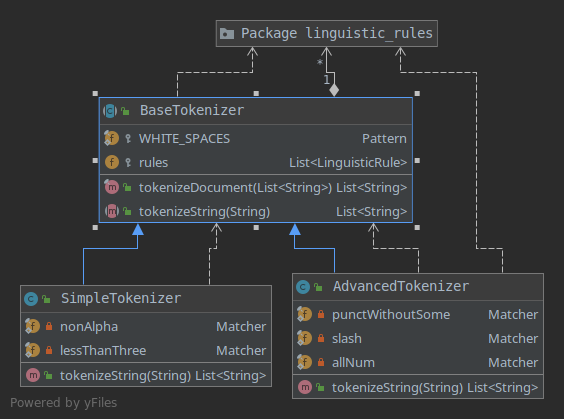
\includegraphics[width=11cm]{packages_tokenizer.png}
  \caption{Diagrama de classes do package \it tokenizer}
\end{figure}

Aqui encontram-se as classes que transformam partes dos documentos em termos (Tokenizers). 
A classe principal, BaseTokenizer, é a classe base das diferentes implementações
de tokenizers. As classes descendestes desta devem implementar o método {\it tokenizeString}
on aplicam regras ao conteúdo recebido, devolvendo uma lista de termos.
Para os tokenizers não existe a noção de documento, simplesmente aplicam regras a
conteúdo recebido.

No nosso tokenizer avançado mantemos as palavras com hífen, eliminamos termos
com apenas dígitos e com menos de 3 caracteres e aplicamos ainda stemming e uma
filtragem de stop words.

\subsubsection{tokenizer.linguestic\_rules}
\begin{figure}[h]
  \center
  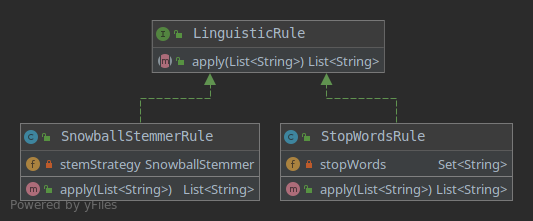
\includegraphics[width=10cm]{packages_tokenizer_linguistic_rules.png}
  \caption{Diagrama de classes do package \it tokenizer.linguistic\_rules}
\end{figure}

De maneira a poder aplicar as mesmas regras em diferentes tokenizers
foi criado uma interface comum que aplica regras linguísticas a termos.
Estas regras linguísticas podem ser, por exemplo, fazer a exclusão se certos termos
que cumprem um conjunto de regras (Stop Words) ou a transformação dos termos (Stemmer).

\subsection{indexer}
\begin{figure}[H]
  \center
  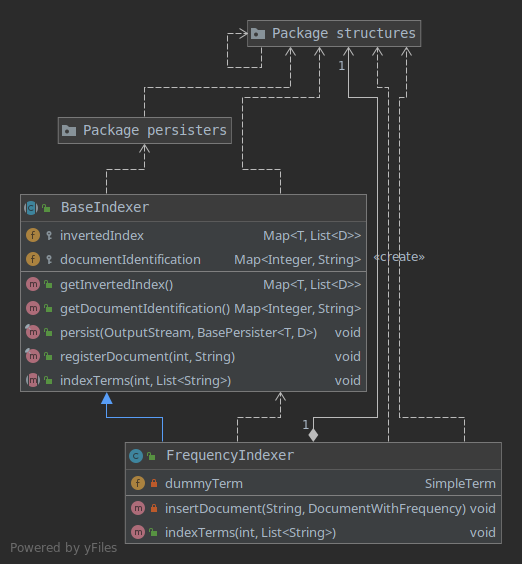
\includegraphics[width=8cm]{packages_indexer.png}
  \caption{Diagrama de classes do package \it indexer}
\end{figure}

Package com as classes que armazenam em memória o index invertido e
a associação entre o id de um documento e o seu identifier.

Aqui está presente a class BaseIndexer que serve como classe base para
diferentes implementações de indexers. O index invertido é guardado numa
estrutura do tipo mapa, permitindo ao programador definir a implementação
desta interface, sendo por defeito usado um HashMap. A classe base referida
é genérica o que possibilita que sejam criados diferentes indexers com a
mesma estrutura, o que leva às classes descendentes a implementar o método
{\it indexTerms} que guarda os termos de um documento no index invertido,
com as estruturas especificas desse indexer.

\subsubsection{indexer.structures}
\begin{figure}[h]
  \center
  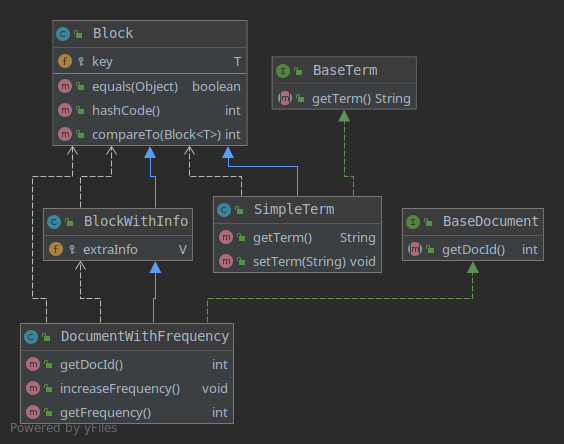
\includegraphics[width=10cm]{packages_indexer_structures.png}
  \caption{Diagrama de classes do package \it indexer.structures}
\end{figure}

Neste package estão os blocos que constroem o index invertido e que permitem
a extensibilidade do mesmo. Tanto a chave do index invertido como o valor presente
na lista associada descende do tipo Block que possui uma key (no caso do termo é o
próprio term e nos documentos o seu id) pela qual é comparável entre si. Em casos
em que seja necessário ter mais informação associada (contagens por exemplo)
a classe BlockWithInfo, descendente de Block, permite isso mesmo.

Para distinguir termos de documentos foram criadas as interfaces BaseTerm e BaseDocument,
logo classes que guardam informação sobre termos devem descender do tipo Block e
implementar a interface BaseTerm e classes que guardam informação sobre documentos
devem descender do tipo Block e implementar a interface BaseDocument.

\subsubsection{indexer.persisters}
\begin{figure}[H]
  \center
  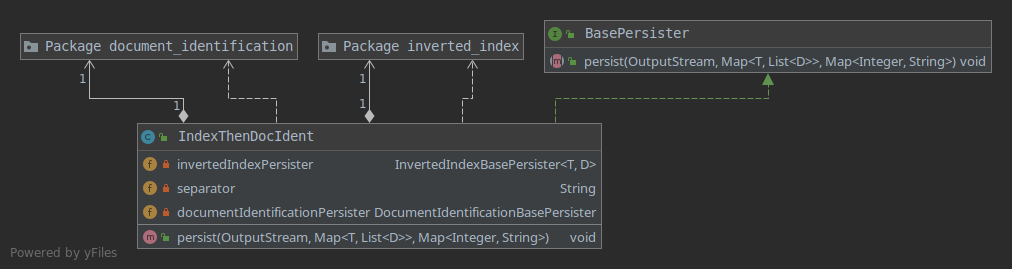
\includegraphics[width=16cm]{packages_indexer_persisters.png}
  \caption{Diagrama de classes do package \it indexer.persisters}
\end{figure}

Aqui encontram-se as classes responsáveis por implementar as diversas
estratégias de guardar as estruturas internas da class BaseIndexer
para disco. Como este indexer apresenta duas estruturas internas,
damos a possibilidade de criar diferentes estratégias para cada
estrutura, assumindo sempre que guardamos para o mesmo ficheiro as
duas estruturas. A classe BaseIndexer, no método {\it persist},
recebe um BasePersister que irá aplicar a estratégia para guardar
ambas as estruturas.

\begin{figure}[h]
  \center
  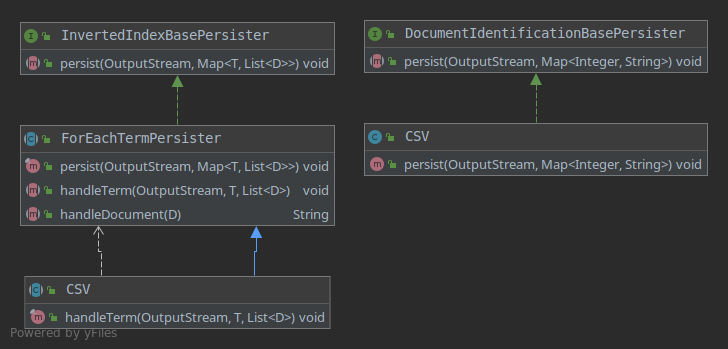
\includegraphics[width=16cm]{packages_indexer_persisters_impl.png}
  \caption{Diagrama de classes do package {\it indexer.persisters.inverted\_index}
  à esquerda e do package \it indexer.persisters.document\_identification
  à direita}
\end{figure}

\newpage

\section{Resultados}

Resultados usando apenas o ficheiro 2004\_TREC\_ASCII\_MEDLINE\_1.gz \\

\begin{tabular}{| p{0.4\linewidth} | p{0.3\linewidth} | p{0.3\linewidth} |}
        \hline
        & \bf SimpleTokenizer & \bf AdvancedTokenizer \\ \hline
        Tempo de indexação (mm:ss) & 3:13 & 2:09 \\ \hline
        Tamanho do index em disco (MB) & 238 & 209 \\ \hline
        Tamanho do vocabulário & 254914 & 427035\\ \hline
        Primeiros 10 termos (em ordem
        alfabética) que aparecem em
        apenas um documento
        &
        aaaa \newline
        aaaai \newline
        aaaasf \newline
        aaaat \newline
        aaab \newline
        aaact \newline
        aaaction \newline
        aaaga \newline
        aaah \newline
        aaahc
        &
        000case \newline
        000diseasegen \newline
        000for \newline
        000g \newline
        000gener \newline
        000iu \newline
        000kb \newline
        000mer \newline
        000meter \newline
        000molecularweight
        \\ \hline
        Dez termos com a maior frequência nos documentos
        &
       and : 1014861 \newline
       the : 1011732 \newline
      with : 311814 \newline
       for : 304357 \newline
      from : 117323 \newline
  patients : 112027 \newline
     human : 106054 \newline
      cell : 90208 \newline
     cells : 85435 \newline
     study : 84058
     &
      cell : 144666 \newline
   patient : 137526 \newline
    effect : 134752 \newline
     human : 109488 \newline
     studi : 106189 \newline
       use : 87725 \newline
     activ : 87489 \newline
       rat : 81501 \newline
    diseas : 79692 \newline
 treatment : 78885
     \\
    \hline
\end{tabular}
\newpage

\section{Anexos}

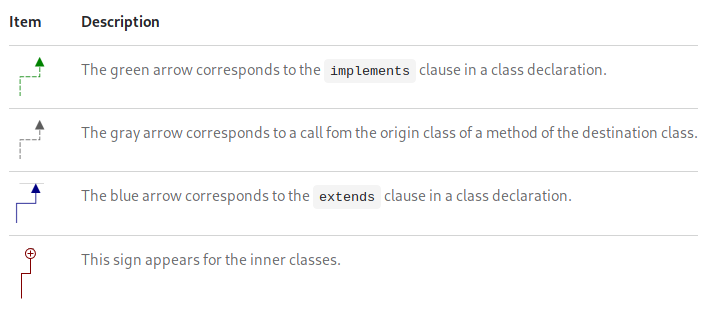
\includegraphics[width=13cm]{arrow_legend.png}

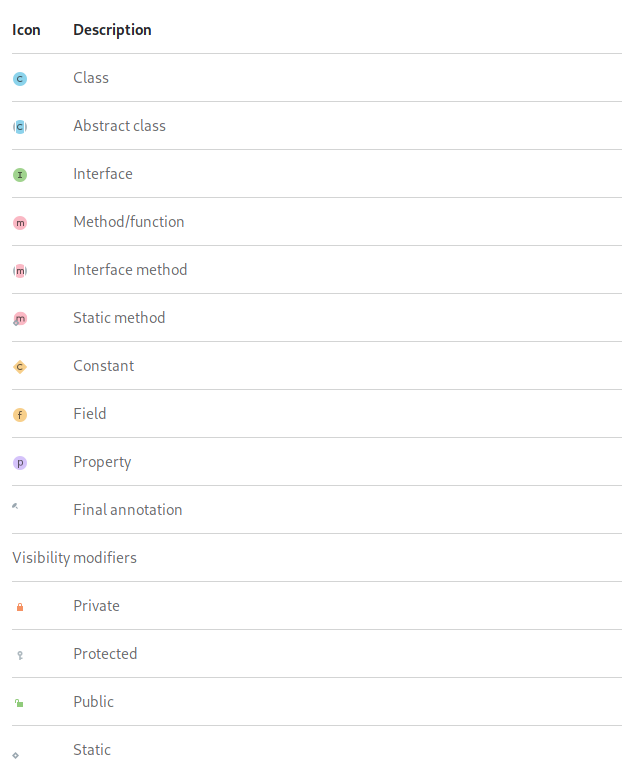
\includegraphics[width=13cm]{icons_legend.png}

\end{document}
